 %%%%%%%%%%%%%%%%%%%%%%%%%%%%%%%%%%%%%%%%%%%%%%%%%%%%%%%%%%%%%%%%%%%%%%%%%%%%%%%%%%%%%
% ITR_LSR_slides class options
% - 'itr' or 'ITR' for ITR version
% - 'lsr' or 'LSR' for LSR version
% - 'german' for a German presentation
% - 'english' for an English presentation (default)
% - 'longpres' if you want to use subsections
% - 'noshadow' if you want to use blocks without shadow
% - 'draftlayout' to show a mm grid as overlay for precise positioning
% - 'presentermode' to generate slides with note-page, usable with e.g. pympress
% - 'coveredhidden' to hide covered objects. Default is transparent.
% beameroptions can be used, e.g.:
% - 'aspectratio=169' for 16:9 wide screen presentations
% - `handout` to generate printable handout sheets
% - `draft` for fast compilation (without graphics)
% do not remove STUDENT option!
%%%%%%%%%%%%%%%%%%%%%%%%%%%%%%%%%%%%%%%%%%%%%%%%%%%%%%%%%%%%%%%%%%%%%%%%%%%%%%%%%%%%%
\documentclass[student, noshadow, lsr, english, aspectratio=169]{ITR_LSR_slides}
\usepackage{tikz}
\usepackage{pgfplots}
\pgfdeclarelayer{background}
\pgfdeclarelayer{nodelayer}
\pgfdeclarelayer{edgelayer}
\pgfdeclarelayer{foreground}
\pgfsetlayers{background,edgelayer,nodelayer,main,foreground}
% robot name for tikz figure
%\newcommand{\RobotName}{$\mathbf{R}$}

\def\CheckAttentionSlide{
    \begin{frame}
        \begin{center}
            {\fontsize{40}{50} \structure{Sorry for your attention}\\}
        \end{center}
    \end{frame}
}

\addbibresource{./refs/mybib.bib}
\graphicspath{{pics/}{logos/}}

\title{Title of Presentation}
\presenter{L. Hochschwarzer}

\supervisor{R. Lefringhausen}
\typeofpres{Intermediate Report / Final Report Master‘s Thesis / Bachelor Thesis}

\usepackage[bigfiles]{media9} %option bigfiles not needed for xelatex, runs without problems on ubuntu14
%%%%%%%%%%%%%%%%%%%%%%%%%%%%%%%%%%%%%%%%%%%%%%%%%%%%%%%%%%%%%%%%%%%%%%%%%%%%%%%%

\begin{document}


\begin{frame}
    \titlepage
\end{frame}


\section{Introduction}
\begin{frame}{Motivation}	
	\begin{columns}[onlytextwidth, T]
		\begin{column}{.5\textwidth}
			\heading{Why are we addressing this problem?}
			\begin{itemize}
				\item<1-> Aaa
				\item<2-> Bbb
				\item<3-> Ccc
			\end{itemize}
		\end{column}
		\begin{column}{.5\textwidth}
			\only<1-2>{\uncovergraphics<2>[height=4cm]{motivation}}
			\only<3>{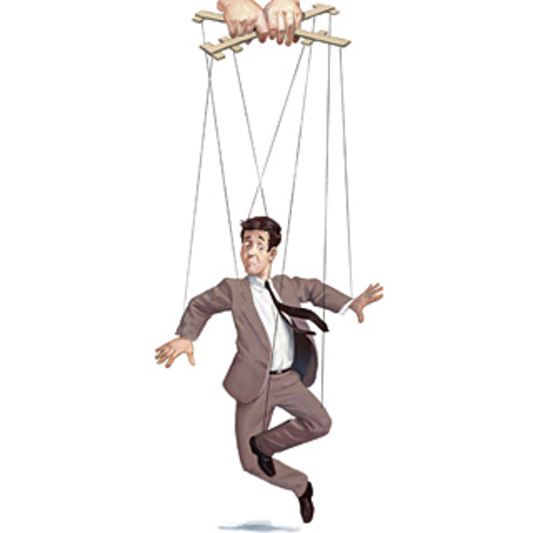
\includegraphics[height=4cm]{control_human}}
		\end{column}
	\end{columns}\vspace{.5cm}
	\uncover<3->{\simpleblock{This is why!}}
	\note{
			Something you should not forgot to mention, that is not part of the slide.
		}
\end{frame}


\begin{frame}
	\frametitle{Related Work}
    Normal cite: \cite{buss11}\\
	Bigger cite: \scite{buss11}\\
	Multiple  authors: \cite[3]{bauer09}
\end{frame}

\section{Methods}

\begin{frame}
	\frametitle{Methods 1}
	\begin{itemize}
		\item a
		\item b
	\end{itemize}
\end{frame}

\begin{frame}
	\frametitle{Methods 2}
	\begin{itemize}
		\item a
	\end{itemize}
\end{frame}

\begin{frame}
	\frametitle{Methods 3}
	\begin{itemize}
		\item a
	\end{itemize}
\end{frame}

\begin{frame}
	\frametitle{Methods 4}
	\framesubtitle{manually positioned blocks}
	
	
	\begin{textblock*}{100mm}(40mm,30mm) 
		\begin{tcolorbox}\color{tum_blue}
			100mm wide at xy={40mm,30mm}
			use document class option `draftlayout' for precise positioning
		\end{tcolorbox}
	\end{textblock*}
	
	\begin{textblock*}{55mm}(100mm,60mm) 
		some positioned text block. 
		Make sure to use the *-Version of textblock for compliance with the grid overlay.
	\end{textblock*}
\end{frame}


\section{Results}

\begin{frame}{Results 1}
	...
\end{frame}

\begin{frame}{Results 2}
	...
\end{frame}

\section[Videos]{Examples for showing videos}
	% VIDEO: both examples below show a figure where the video will be displayed. 
	% This figure could be a still picture of the video, giving a hint on what the video will show. 
	% Usage of such a figure can be useful in case the presentation is likely to be printed as e.g. a handout 
	
	% NOTE: the folder containing the videos MUST BE INSIDE the presentation folder, otherwise the videos might not show up in the presentation.
	% Also: the videos cannot be displayed on ubuntu, use e.g. the windows imperator to check whether the videos work
	
	% The videos need to be converted to swf format. See the wiki for a procedure to convert videos from mp4 to swf: https://wiki.lsr.ei.tum.de/groups/iuro/videocoding?s[]=avconv
	
	%video example swf
	{
		\begin{frame}[plain]
			\includemedia[width=12.8cm,height=9.6cm,activate=onclick,]{
				
\includegraphics{motivation}
			}{movie/example_video_short.swf}
		\end{frame}
	}
	
	%video example mp4 (tested on ubuntu ubuntu 20.04 using okular )
	\begin{frame}{mp4 Video in pdf (using Okular)}
		\includemedia[
		width=6cm, keepaspectratio,
		activate=pageopen,
		transparent,
		addresource=movie/OTG_simulation.mp4,
		flashvars={
			source=movie/OTG_simulation.mp4
			&autoPlay=true       % start playing on activation
			&loop=true % start again when finished
		}
		]{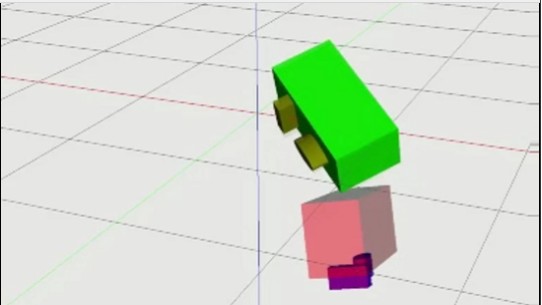
\includegraphics{movie/OTG_simulation}}{VPlayer.swf}
	\end{frame}
	
	% only worth testing via pympress in presentermode
	\begin{frame}{mp4 video in pympress}
		\begin{textblock*}{90mm}(40mm,66mm) 
			\begin{tcolorbox}\color{tum_blue}
				\centering
				This frame will only show a video, if you use 
				\href{https://pympress.readthedocs.io/en/latest/README.html}{\textbf{pympress}}
				 (you may also want to add the `presentermode` option)
			\end{tcolorbox}
		\end{textblock*}
		\movie[autostart,poster]{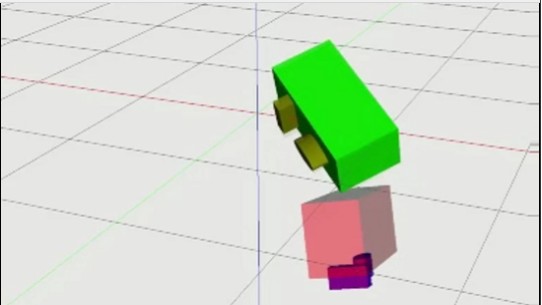
\includegraphics[width=6cm,keepaspectratio]{movie/OTG_simulation.png}}{movie/OTG_simulation.mp4}
		\note{
			\textbf{autostart is currently not supported! Click video in presenter mode to start video}
		}
	\end{frame}
	
	% robust version use external player
	\begin{frame}{mp4 Video in external player}	 
		\href{run:movie/OTG_simulation.mp4}{
			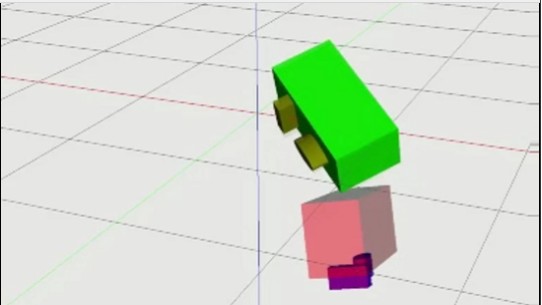
\includegraphics[width=6cm,keepaspectratio]{movie/OTG_simulation.png}
		}
	\end{frame}
	
\section{Summary}

\begin{frame}{Summary}
	...
\end{frame}

	\appendix
	% This slide serves 3 purposes:
	% 	1. a simple example how to create figures in tikz using beamer
	%	2. testing if you actually checked the content of this template
	% 	3. subtly preventing you from adding a "Thank you..." slide at the end of your presentation
	% If this slide is still in your final presentation... well, congratulation!
	\CheckAttentionSlide


%\nocite{buss11}
%\nocite{bauer09}
\begin{frame}{\LSRITRRefTitle}
	\printbibliography
\end{frame}


\end{document}
